\documentclass[10pt]{beamer}

\usepackage[utf8]{vietnam}
\usetheme[secheader]{Boadilla}
\usecolortheme{beaver}
\usefonttheme{professionalfonts}


\usepackage{textpos}
\usepackage{tikz}
\usepackage{graphicx}
\usepackage{xcolor}
\useoutertheme[red,subsection=false]{smoothbars}
%\useoutertheme{smoothtree}
%\logo{
\includegraphics[width=0.7cm]{Figs/fig}\vspace{200pt}}



\tikzstyle{startstop} = [rectangle, rounded corners, text width=3cm, minimum height=1cm,text centered, draw=red, fill=red!60]
\tikzstyle{io} = [trapezium, trapezium left angle=70, trapezium right angle=110, minimum width=3cm, minimum height=1cm, text centered, draw=black, fill=blue!30]
\tikzstyle{process} = [rectangle, text width=3cm, minimum height=1cm, text centered, draw=orange, fill=orange!60]
\tikzstyle{decision} = [diamond, minimum width=3cm, minimum height=1cm, text centered, draw=black, fill=green!30]
\tikzstyle{arrow} = [thick,->,>=stealth]



\definecolor{redd}{RGB}{207,22,40}
\definecolor{yello}{RGB}{243,195,9}

\setbeamercolor*{subitem projected}{fg = yello, bg = redd}%
\setbeamercolor*{structure}{fg = redd}%

\setbeamertemplate{itemize items}{\normalsize$\bullet$} 
\setbeamertemplate{enumerate items}[circle] 
\setbeamertemplate{sections/subsections in toc}[circle]


\pgfdeclareimage[height=\paperheight,width=\paperwidth]{bgimage}{Figs/bg.jpg}
\usebackgroundtemplate{\tikz\node[opacity=0.1,inner sep=0]{\pgfuseimage{bgimage}};}

\title[Đánh giá năng suất]{Học phần: \textbf{Quản Lý Sản Xuất}}
\subtitle{EM3417 - 20201 - 119636}
\author[EM3417 - 20201 - 119636]{\large {\textbf{Chủ đề: Đánh giá năng suất}}}
\institute[Nhóm 2]{\large {Nhóm 2}}
\date{\today}

\beamertemplatetransparentcoveredhigh
\begin{document}

\frame{\titlepage\transsplitverticalout}

\addtobeamertemplate{frametitle}{}{%
\begin{textblock*}{100mm}(.95\textwidth,-0.8cm)

\includegraphics[width=0.6cm]{Figs/fig}
\end{textblock*}}








\begin{frame}
\label{contents}
\transblindshorizontal
\frametitle{\textbf{Nội dung}}
\tableofcontents
\end{frame}


\section{Đặt vấn đề}
\begin{frame}
\transsplitverticalout
\frametitle{Đặt vấn đề}
%\framesubtitle{The proof uses \textit{reductio ad absurdum}.}
\begin{figure}
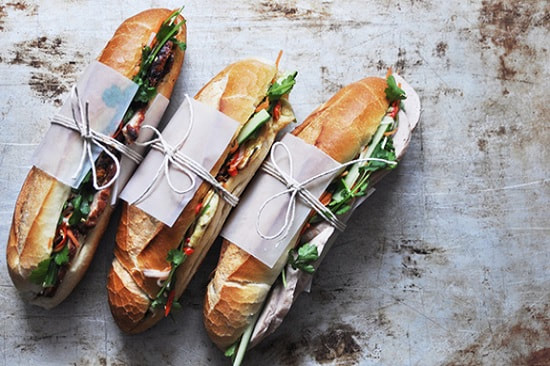
\includegraphics[scale=0.2]{Figs/banhmi.jpg}
\end{figure}

\begin{block}{Tiệm bánh mỳ của Trường}
Tiệm bánh mỳ của Trường có một nhà máy sản xuất thịt nướng. Trong thời
gian qua, Trường nhận ra rằng nhà máy của mình đã sản xuất quá nhiều trong khi lượng
tiêu thụ bánh mỳ thịt nướng lại không cao. Từ đó, Trường muốn biết công suất của
nhà máy nên là bao nhiêu là hợp lý.
Và Trường muốn hiểu hơn nữa về năng suất của hiệu bánh, muốn biết nên có bao nhiêu máy để đạt mức công suất đã hoạch định, những yếu tố nào có thể ảnh hưởng đến việc quyết
định năng suất của tiệm bánh?
\end{block}

\begin{enumerate}
\item Tại sao tiệm bánh mỳ lại gặp phải những khó khăn này?
\item Làm thế nào để nâng cao hiệu quả sử dụng máy móc?
\end{enumerate}

\end{frame}


\section{Tổng quan về năng suất}


\subsection{Khái niệm}
\begin{frame}
\transsplitverticalin
\frametitle{Khái niệm về năng suất}
%\framesubtitle{Trong quản trị sản xuất.}

\begin{figure}

\includegraphics[scale=0.5]{Figs/khainiem}
\end{figure}

Năng suất/năng lực sản xuất là khả năng sản xuất của máy móc, thiết bị, lao động và
các bộ phận của doanh nghiệp trong trong một đơn vị thời gian nhất định (tháng, quý,
năm...) trong điều kiện xác định.

\end{frame}

\subsection{Phân loại năng suất}
\begin{frame}
\transsplitverticalout
\frametitle{Phân loại năng suất}

\begin{itemize}
\item Năng suất dự định: Đầu ra cực đại của một quy trình trong điều kiện hoàn hảo.
\item Năng suất hiệu quả: Đầu ra cực đại của một quy trình trong điều kiện thông thường.
\item Năng suất thực tế: Khối lượng sản phẩm doanh nghiệp đạt được trong
thực tế.
\end{itemize}
Ba khái niệm trên có ý nghĩa rất quan trọng. Chúng được sử dụng để xác định hai chỉ tiêu mức độ hiệu quả và mức độ sử dụng của năng suất:\\
\begin{center}
Mức hiệu quả $= \frac{P_{tt}}{P_{hq}} \times 100\%$\footnote{$P_{tt}$:Năng suất thực tế, $P_{hq}$:Năng suất hiệu quả}\\

Mức độ sử dụng $= \frac{P_{tt}}{P_{dd}} \times 100\%$\footnote{$P_{dd}$:Năng suất dự định}
\end{center}

\end{frame}


\section{Đánh giá năng suất}

\subsection{Các nhân tố tác động đến năng suất}
\begin{frame}{Các nhân tố tác động đến năng suất}
\transsplitverticalout


\begin{tikzpicture}[node distance=2cm]
\node (bai3) [startstop] {CÁC NHÂN TỐ ẢNH HƯỞNG ĐẾN NĂNG SUẤT};
\node (pp1) [process, below of=bai3, yshift=5cm] {\textbf{Tình hình thị trường}: Nhu cầu, cạnh tranh, giá cả, chất lượng};
\node (pp2) [process, below of=bai3, yshift=-0.5cm] {\textbf{Vốn}: Nguồn cung cấp, cơ cấu, tình hình tài chính};

\node (pp3) [process, right of=bai3, xshift = 2cm] {\textbf{Khả năng và tình hình tổ chức sản xuất}: Quy mô, chuyên môn hoá
, liên kết kinh tế};
\node (pp4) [process, right of=bai3, xshift = 2cm, yshift=3cm] {\textbf{Cơ chế quản lý và chính sách vĩ mô}: Chính sách đối
ngoại, chính sách cơ cấu kinh tế};
\node (pp5) [process, right of=bai3, xshift = 2cm, yshift=-2.5cm] {\textbf{Công nghệ}: Máy móc thiết bị, nguyên liệu, quá trình};

\node (pp6) [process, left of=bai3, xshift=-2cm] {\textbf{Trình độ quản lý}: Đội ngũ cán bộ quản lý, cơ cấu thứ bậc, cơ chế hoạt động};
\node (pp7) [process, left of=bai3, xshift=-2cm, yshift=3cm] {\textbf{Môi trường kinh tế thế giới}: Tình hình kinh
tế thế giới, hội nhập quốc tế, tình hình các nguồn lực};
\node (pp8) [process, left of=bai3, xshift=-2cm, yshift=-2.5cm] {\textbf{Lao động}: Số lượng, chất lượng, trình độ tay
nghề, chuyên môn};

%\node (bdmt) [startstop, below of=bai3, xshift=-3cm, yshift=6cm] {Nhập ma trận A, b};
%\node (a) [startstop, below of=bai3, xshift=3cm, yshift=6cm] {Kiểm tra tính chéo trội};

%\node (hpt) [startstop, left of=bai3, xshift=-4cm, yshift=-1cm] {Tính nghiệm gần đúng, sai số};
%\node (ngd) [startstop, right of=bai3, xshift = 3cm, yshift=-1cm] {Kiểm tra sự hội tụ};


\draw [arrow] (bai3) -- (pp1);
\draw [arrow] (bai3) -- (pp2);
\draw [arrow] (bai3) -- (pp3);
\draw [arrow] (bai3) -- (pp4);
\draw [arrow] (bai3) -- (pp5);
\draw [arrow] (bai3) -- (pp6);
\draw [arrow] (bai3) -- (pp7);
\draw [arrow] (bai3) -- (pp8);
%\draw [arrow] (bai3) -- node[anchor=south] {(4)} (hpt);
%\draw [arrow] (bai3) -> node[anchor=east] {(1)} (bdmt);
%\draw [arrow] (bai3) -- node[anchor=south] {(3)} (ngd);
%\draw [arrow] (bai3) -- node[anchor=east] {(2)} (a);
\end{tikzpicture}

\end{frame}

\subsection{Bản chất và tầm quan trọng của năng suất trong sản xuất và dịch vụ}
\begin{frame}
\transsplitverticalout
\frametitle{Bản chất và tầm quan trọng của năng suất}
\framesubtitle{Trong sản xuất và dịch vụ.}




\end{frame}

\subsection{Những biện pháp nhằm nâng cao năng suất trong quản trị sản xuất}
\begin{frame}
\transsplitverticalout
\frametitle{Những biện pháp nhằm nâng cao năng suất}
\begin{figure}

\includegraphics[scale=0.3]{Figs/nangcao}
\end{figure}
Năng suất phụ thuộc chặt chẽ vào khả năng thiết kế và tổ chức điều hành hệ thống sản
xuất. Do vị trí, vai trò của năng suất hết sức quan trọng đối với sự tồn tại phát triển và
khả năng cạnh tranh của doanh nghiệp, vì vậy nâng cao năng suất là nhiệm vụ quan
trọng hàng đầu trong quản trị sản xuất. 


\end{frame}

\begin{frame}
\transsplitverticalout
\frametitle{Những biện pháp nhằm nâng cao năng suất}
Một số biện pháp nhằm nâng cao năng suất trong doanh nghiệp gồm: 
\begin{enumerate}
\item Xây dựng hệ thống các chỉ tiêu và thước đo năng suất đối với tất cả các hoạt động tác
nghiệp. Đây là nhiệm vụ quan trọng nhưng hiện nay Việt nam vẫn chưa có hệ thống chỉ tiêu
thống nhất đánh giá năng suất theo cách tiếp cận mới, hội nhập với khu vực và thế giới.
\item Xác định rõ mục tiêu hoàn thiện năng suất trong sản xuất. Căn cứ vào hệ thống sản
xuất hiện tại và tình hình thực hiện các mục tiêu kế hoạch sản xuất để lựa chọn mục tiêu hợp lý.
\item Phân tích, đánh giá quá trình sản xuất phát hiện những khâu yếu nhất để có những biện pháp khắc phục. Đây là khâu quyết định đến năng suất của toàn bộ hệ thống
sản xuất.
\item Cải tiến kỹ thuật và đổi mới công nghệ.
\end{enumerate}

\end{frame}

\section{Lựa chọn năng suất}

\subsection{Subsection 1}
\begin{frame}
\transsplitverticalout
\frametitle{Title 6}





\end{frame}


\subsection{Subsection 2}
\begin{frame}
\transblindshorizontal
\pause
\frametitle{Title 7}

\end{frame}

\begin{frame}{Title 8}
\transsplitverticalin
\centering
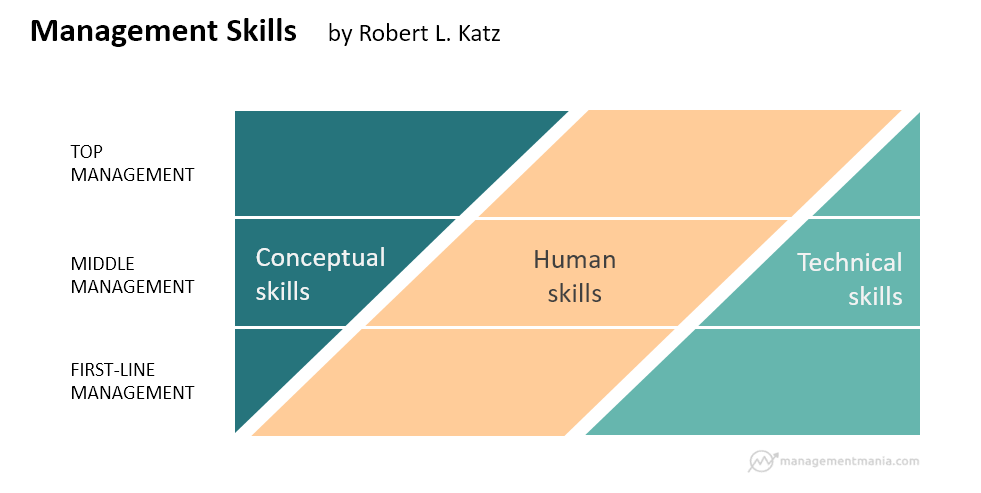
\includegraphics[scale=0.4]{Figs/fig6}
\end{frame}

\subsection{Subsection 3}
\begin{frame}
\transsplitverticalout
\frametitle{Title 9}

\end{frame}

\begin{frame}
\transblindshorizontal
\frametitle{Title 10}

\end{frame}

\begin{frame}
\transsplitverticalin
\frametitle{Title 11}

\end{frame}

\begin{frame}
\transsplitverticalout
\frametitle{Title 12}

\end{frame}






    
\section*{Kết}
\begin{frame}
\transsplitverticalin
\centering
\begin{tabular}{|c||c|}
\hline 
\textbf{Thành viên} & \textbf{MSSV} \\ 
\hline 
Nguyễn Trần Thức  & \textit{20185483} \\ 
\hline 
Đỗ Đức Chung & 20171019 \\ 
\hline 
Vũ Đăng Chiến  & 20172432 \\ 
\hline 
Cao Ngọc Đông 
(Nhóm Trưởng)
 & 20161020 \\ 
\hline 
\end{tabular}
\\
\centering
{\fontsize{40}{50} \textcolor{redd}{\textbf{Thank You!}}}

\hyperlink{contents}{\beamerbutton{Contents page}}
\end{frame}

\begin{frame}
\transsplitverticalout
\centering
{\fontsize{40}{50} \textcolor{redd}{\textbf{Q \& A}}}
\end{frame}


\end{document}